\subsection{Visualiser and REST Server}\label{ssec:rest-server}

    \subsubsection{Overview and Analysis}
        Diagrams produced by the above sections were visualised as graphs of nodes and edges within an SVG (scalable vector graphic).
        Further, this graph was made interactive using ECMAScript's d3.js library, in particular using force-directed graphs.
        This was coupled through a back-end server acting as a reduction engine with a representational state transfer (REST) architecture and a front-end webpage with ECMAScript components for interacting with the output of the server.\\

        The REST server was a single endpoint with options of GET and POST requests.
        GET returned an example diagram as a JSON object --- in particular, this was a collection of four disconnected diagrams, one for each type of edge reduction.
        POST would, given a JSON object, reduce and return a new diagram.
        
        \begin{remark*}{Cross-Origin Resource Sharing (CORS)\\}
            As a note on the bureaucracy of various web standards, the implementation written for this project involved making cross-origin HTTP requests.
            By default, this behaviour is not allowed, so an additional CORS layer is wrapped around the server to allow such requests.
        \end{remark*}~

        The front-end visualisation was, in comparison, far more complex.
        To begin, there would be a GET request to the REST server for the default diagram.
        The returned JSON object was parsed to an SVG.
        In particular, SVG groups were made of edges, nodes and boxes.
        Each class of edge, node and box contained a set of polylines, a circle and a collection of both nodes and edges respectively.
        Nodes were coloured depending upon the property of their position relative to boxes: external, perimeter or internal.\\

        Interactivity was added using an ECMAScript script and additionally a `Reduce' button.
        Each node was made draggable and forces were added to each node and edge.
        In particular:
        \begin{itemize}
            \item Edges were given spring forces to allow them to stretch on drag actions and contract to a relaxed length otherwise.
            \item Nodes were given repulsive charges to allow them to spread themselves out evenly over the available space.
            \item The graph as a whole was given a small central attractive charge to keep the graph centered in the viewing panel.
        \end{itemize}
        The `Reduce' button would then make a POST request to the REST server to update the current graph dataset with its reduction.\\

        Due to the multiple paradigms and flexibility of the language, a small excerpt of code can be found in~\ref{ssec:appendix-graph-source}.
        In particular, this utilises a functional programming style --- the algorithm amounts to multiple filter-map-reduce operations on the dataset.
        For example, graph edges (links) are added through the following method:
        \begin{itemize}
            \item Create an SVG group for all edges
            \item Select all current and new edges
            \item Create an SVG group for each edge
            \item Select all sub-edges to each edge (one sub-edge for the subject node, then one for each object node)
            \item Create a polyline for each sub-edge
        \end{itemize}

        The filter operation is only necessary to manage discrepancies in how nodes are partitioned into those in boxes and those not.
        The naive method would be to gather the sets of nodes referenced in each graph's set of edges, but this has its problems.
        Principal nodes on the perimeter of boxes will be included both within their respective box and in the surrounding graph (unless the box is disconnected).
        For this reason, principal nodes are considered part of the parent graph --- consider the case of two boxes sharing a principal node, this requires the principal to either be in both boxes or in the parent graph.
        Furthermore, when black box styles are drawn around diagram boxes, nodes on the perimeter may be outside the box as drawn, but the end of the polyline connecting the node to the internal graph must stay in the drawn box.
        This leaves perimeter nodes sitting precisely on the perimeter, neither wholly inside or out.\\

        On the event of a reduction being requested, the above creates a new SVG.
        This leaves new nodes inheriting a default position, visually manifested as a `jump' of all nodes to the origin $(0, 0)$ in the top-left corner.
        This is not particularly appealing, so additionally when a new set of nodes and edges is received, positions are copied over where the unique id of nodes match one another.
        While only a small detail, this change leads to visually `smooth' reductions and is far more intuitive as to what is happening within the graph.


    \subsubsection{Testing and Correctness}
        The particularly clear and interactive nature of the diagrams, coupled with the difficulty of constructing an $\alpha$-equivalence algorithm (graph isomorphism) led to testing being conducted visually.
        The following exhibits the reduction of some simple diagrams.
        While the palette of colours used is fixed, the choice of which colour is assigned to which property is not fixed, so colours do change between examples.

        \begin{examples}{~\\}\label{sssec:diagram-reductions}
            The first case here shows a normal fusion across two edges.
            The arrowheads represent the parity of the edge and, in implementation but not shown here, there exist mouseover text boxes with the name of the node if it exists.
            What should be notable is the potential ambiguity behind this visualisation --- the repeated object within an edge is non-obvious aside from a very slight difference in darkness of the line.
            \begin{figure}[H]
                \centering
                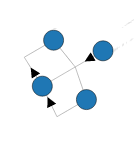
\includegraphics[width=0.2\textwidth]{diagrams/edge-edge.png}
                \hspace{1in}
                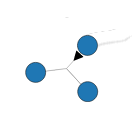
\includegraphics[width=0.2\textwidth]{diagrams/edge-edge-reduction.png}
                \caption*{$(a \, c)(\bar{b} \, a \; | \; b \, c \; | \; p \, a \, b \, c) \quad \rightarrow \quad (x)(p \, x \, b \, x)$}
            \end{figure}~\\
                        
            This case demonstrates a reduction between an edge and a box.
            This exhibits both how perimeter nodes lie exactly on the perimeter, while internal nodes lie entirely inside.
            The use of colours also makes clear the position of each node relative to the box.
            \begin{figure}[H]
                \centering
                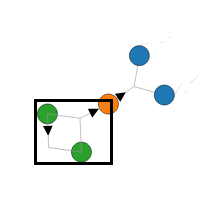
\includegraphics[width=0.3\textwidth]{diagrams/edge-box.png}
                \hspace{0.5in}
                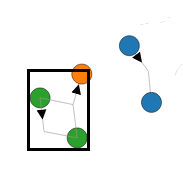
\includegraphics[width=0.3\textwidth]{diagrams/edge-box-reduction.png}
                \caption*{$(!(x \, y)(\bar{u} \, x \, y \; | \; x \, y) \; | \; u \, a \, b) \quad \rightarrow \quad (!(x \, y)(u \, x \, y \; | \; x \, y) \; | \; a \, b)$}
            \end{figure}~\\
           
            Again the diagram demonstrates how the colours change around boxes, but here on a internal box reduction.
            This, like the next diagram, could be reduced ad-infinitum, but such effect will be shown later.
            In particular, this demonstrates the explicit creation of new nodes, but again there is ambiguity in the number of objects of the newly created edge (two objects, not one).
            \begin{figure}[H]
                \centering
                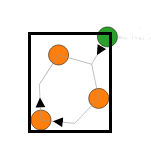
\includegraphics[width=0.22\textwidth]{diagrams/intra-box.png}
                \hspace{1in}
                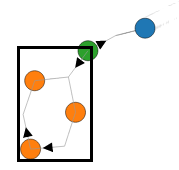
\includegraphics[width=0.28\textwidth]{diagrams/intra-box-reduction.png}
                \caption*{$!(a \, b)(\bar{x} a \; | \; x \, b \; | \; p \, a \, b) \quad \rightarrow \quad (!(a \, b)(\bar{x} a \; | \; x \, b \; | \; p \, a \, b) \; | \; (x) \, p \, x \, x)$}
            \end{figure}~\\
            
            Completing the set of cases of fusions, an example of a reduction between two boxes, demonstrating the non-finite nature of the reductions.
            Like the first example, there exists some ambiguity as to the order of objects across a node --- there is no obvious way to tell which combination of pairs two edges are matching together.
            In a larger context the distinction is usually more obvious, but the presence of such ambiguity is recognised to be a shortfall.
            \begin{figure}[H]
                \centering
                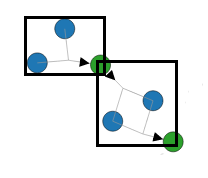
\includegraphics[width=0.25\textwidth]{diagrams/box-box.png}
                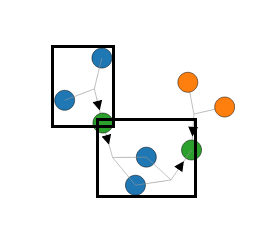
\includegraphics[width=0.3\textwidth]{diagrams/box-box-reduction.png}
                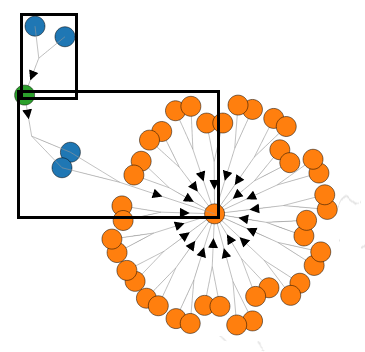
\includegraphics[width=0.25\textwidth]{diagrams/box-box-many-reduction.png}
                \caption*{$(!(a \, b)(u \, a \, b) \; | \; !(c \, d)(\bar{u} \, c \, d \; | \; w \, c \, d)) \quad \rightarrow \quad (!(a \, b)(u \, a \, b) \; | \; !(c \, d)(\bar{u} \, c \, d \; | \; w \, c \, d) \; | \; (x \, y) \, w \, x \, y \; | \; \ldots \;)$}
            \end{figure}~\\
                        
            Together, these diagrams may be reduced one after the other.
            A full chain of step-by-step reductions can be found in~\ref{ssec:appendix-diagram-reduction}.
            \begin{figure}[H]
                \centering
                \begin{subfigure}{0.4\linewidth}
                    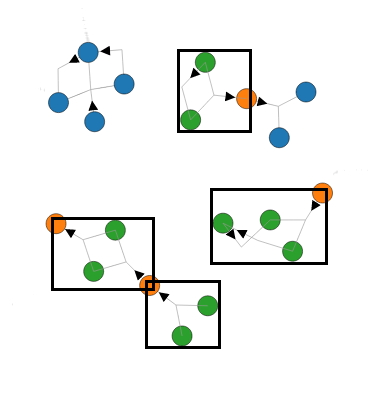
\includegraphics[width=\textwidth]{diagrams/all-diagrams.png}
                \end{subfigure}
                $\longrightarrow^{*}$
                \begin{subfigure}{0.4\linewidth}
                    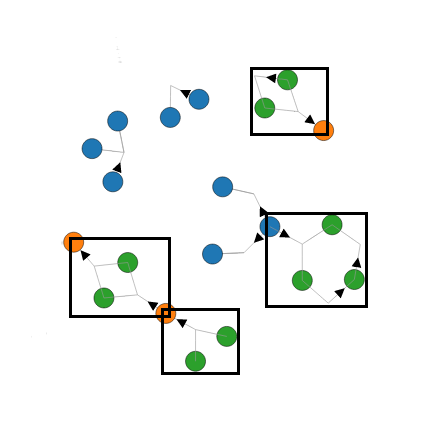
\includegraphics[width=\textwidth]{diagrams/all-diagrams-r4.png}
                \end{subfigure}
            \end{figure}
        \end{examples}


    \subsubsection{Discussion}
        While the final example may not seem like a full reduction as the box-box diagram has not reduced, the choice of whether to reduce the internal box example or the box-box is not `fair'.
        That is, there is no guarantee that a given reduction will be performed if there exists a non-finite chain of reductions that may be performed instead.
        This behaviour is not ideal, but isn't necessarily incorrect.
        Should there be further development, this effect should be addressed early.
        In the case of reductions involving only boxed edges, alternative behaviour could be defined to check whether the set of nodes after a reduction differs from the set before a reduction.
        In this way, while not compromising the multiset properties of diagrams, the pitfalls may be avoided --- the reduction may be performed again, but only once the residue of the last reduction has been affected.\footnotemark
        \footnotetext{This is not a perfect solution still as one can build a similar infinite loop between two repeated reductions that interact with one another etc\ldots}
        Further options would include performing multiple reductions across the diagram as a whole in one step, ensuring that every reduction that can be performed will be performed.
        Unfortunately, this will lead to excessive reductions on such non-finite subdiagrams.
        \textit{I believe this area more than most is still requiring further research and development.}\\

        The multiple cases of ambiguity leave something to be desired.
        From a UX point of view, the implementation is lacking here, \textit{but I have yet to find a suitable improvement}.
        Nodes could be discreetly numbered or labeled to describe their order in the list of objects of an edge, however this numbering will differ on an edge-by-edge basis.
        Numbering or labelling edges would be ideal, however the decisions made in development would make such a feature difficult to introduce.
        The issues with repeated objects in the same edge could be improved by adding extra shape to the lines drawn.
        As the line is drawn as a single line segment from the hidden `connection' node of the edge to the object, adding an extra node between the two, along with the static repulsion of all nodes, would clearly demonstrate nodes with multiple occurrences in a single edge's objects.
        Alternatively, given a labelling of the index of a node in an edge's objects as suggested formerly, this could further be a set of indices for each occurrence.
        \begin{example*}{Improvements to Labelling of Edges and Objects\\}
            \begin{figure}[H]
                \centering
                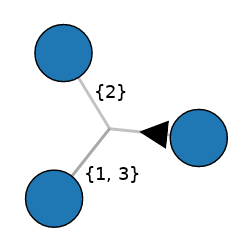
\includegraphics[width=0.25\textwidth]{diagrams/diagram-large.png}
            \end{figure}
        \end{example*}
